\baitndungsai{De01DS:01}{
	Trong không gian $Oxyz$, cho ba điểm $A(2;-1;1)$, $B(-1;3;-1)$ và $\overrightarrow{u}=(1;2;3)$. Xét tính đúng, sai của các khẳng định sau:
}{\bonpatest
	{\TFTrue Tọa độ véc tơ $\overrightarrow{AB}$ là $(-3;4;-2)$.}
	{Tọa độ điểm $C$ để $\overrightarrow{AC}=\overrightarrow{u}$ là $(3;3;4)$}
	{Tọa độ trung điểm $I$ của $AC$ là $(5;0;5)$.}
	{\TFTrue Tọa độ điểm $D$ để $ABCD$ là hình bình hành là $(6,-3,6)$.}
}{
	Nội dung lời giải
}

\baitndungsai{De01DS:02}{
	Cho hàm số $y=\frac{-x^{2}-3x+4}{x-3}$ có đồ thị $(C)$. Xét tính đúng sai của các mệnh đề sau:
}{\bonpatest
	{\TFTrue Đồ thị $(C)$ có đường tiệm cận xiên là $y=-x-6$.}
	{\TFTrue Đồ thị $(C)$ nhận điểm $I(3;-9)$ làm tâm đối xứng.}
	{Hàm số $y=f(x)$ đã cho đồng biến trên $(3;7)$.}
	{\TFTrue Đồ thị $(C)$ có hai điểm cực trị nằm ở hai phía đối với trục $Oy$.}
}{
	
}

\baitndungsai{De01DS:03}{
	Cho hàm số $f(x)=\frac{2x^{3}+3x+7}{x-1}$. Xét tính đúng sai của các khẳng định sau:
}{\bonpatest
	{$\lim\limits_{x\to -1^{+}}f(x)=-\infty$.}
	{\TFTrue Đường thẳng $x=-1$ là đường tiệm cận đứng của đồ thị hàm số.}
	{\TFTrue $\lim\limits_{x\to -\infty}\frac{f(x)}{x}=2$.}
	{\TFTrue Đường thẳng $y=2x+1$ là tiệm cận xiên của đồ thị hàm số.}
}{
	
}

\baitndungsai{De01DS:04}{
	Cho hàm số $f(x)=\sqrt{1-x}+\sqrt{1+x}$. Xét tính đúng sai của các khẳng định sau:
}{\bonpatest
	{\TFTrue Tập xác định của hàm số đã cho là $\mathbb{D}=[-1;1]$.}
	{Đạo hàm của hàm số đã cho là $f'(x)=\frac{\sqrt{1-x}-\sqrt{1+x}}{2\sqrt{1-x^{2}}}$ với mọi $x\in (-1;1)$.}
	{$\min\limits_{[-1;1]}f(x)=f(0)$.}
	{$\min\limits_{[-1;1]}f(x)+\max\limits_{[-1;1]}=2$.}
}{
	
}

\baitndungsai{De01DS:05}{
	Cho hàm số $y=f(x)$ xác định liên tục trên $\mathbb{R}$ và có bảng xét dấu đạo hàm như sau:
	
	\centerline{
		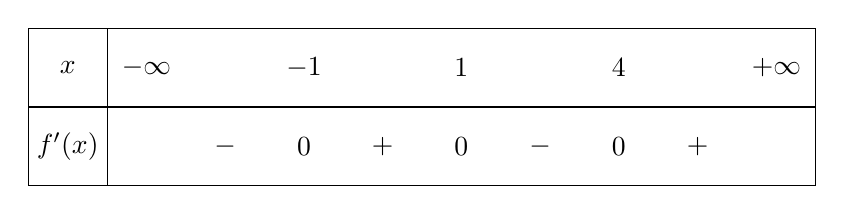
\begin{tikzpicture}
			\foreach \x/\gt in {0/x,1/-\infty,3/-1,5/1,7/4,9/+\infty}\path (\x,0) node{$\gt$};
			\foreach \x/\gt in {0/f'(x),2/-,3/0,4/+,5/0,6/-,7/0,8/+}\path (\x,-1) node{$\gt$};
			\draw (-.5,.5) rectangle (9.5,-1.5) (-.5,-.5)--(9.5,-.5) (.5,.5)--(.5,-1.5);
		\end{tikzpicture}
	}
	
	Xét tính đúng, sai của các khẳng định sau:
}{\bonpatest
	{\TFTrue Hàm số đã cho đồng biến trên các khoảng $(-1;1)$ và $(4;+\infty)$.}
	{Hàm số đạt cực đại tại $x=4$.}
	{\TFTrue $f'(x)=0\Rightarrow \left[\begin{array}{l} x=-1 \\ x=1 \\ x=4\end{array}\right.$.}
	{\TFTrue Hàm số đã cho có $2$ điểm cực tiểu.}
}{
	
}

\baitndungsai{De01DS:06}{
	Cho hình chóp $S.ABCD$ có đáy $ABCD$ là hình chữ nhật, cạnh bên $SA$ vuông góc với mặt phẳng đáy. Gọi $I$ là giao điểm của $AC$ và $BD$ Các khẳng định sau đúng hay sai?
}{\bonpatest
	{\TFTrue $\overrightarrow{SA}+\overrightarrow{SC}=2\overrightarrow{SI}$.}
	{\TFTrue $\overrightarrow{BC}\cdot\overrightarrow{SC}=\overrightarrow{AC}\cdot\overrightarrow{BC}$.}
	{$\overrightarrow{SA}+\overrightarrow{SC}=\overrightarrow{SB}+\overrightarrow{SD}$.}
	{$\overrightarrow{SA}-\overrightarrow{SI}=\overrightarrow{SI}-\overrightarrow{SB}$.}
}{
	
}

\baitndungsai{De01DS:07}{
	Một vật được ném ngang từ độ cao $4$ mét chuyển động theo hình dạng parabol có phương trình $h(t)=-at^{2}+4$  trong đó $t$ là thời gian (tính bằng giây), $h(t)$ là độ cao của vật tại thời gian $t$ (tính bằng mét). Biết  rằng tính từ thời gian vật bắt đầu chuyển động đến khi vật chạm đất là $4$ giây. Xét tính đúng sai của các khẳng định sau:
}{\bonpatest
	{\TFTrue Giá trị của hệ số $a$ là $a=\frac{1}{4}$.}
	{\TFTrue Tốc độ của vật tại thời điểm $t=2$ (giây) là $1$ ($m/s$).}
	{\TFTrue Tại thời điểm $t=2$ (giây) vật có độ cao là $h=2$ (mét).}
	{Nếu cùng lực ném ban đầu và nâng độ cao lên $8$ mét thì sau $4$ giây vật vẫn chạm đất.}
}{
	
}



